
\documentclass[12pt]{article}
\usepackage{setspace}
\doublespacing
\usepackage{fullpage}
\usepackage{amsbsy}
\usepackage{amsmath}
\usepackage{amsfonts}
\usepackage{amsthm}
\usepackage{amssymb}
\usepackage{algorithmic}
\usepackage{algorithm}
\usepackage{enumerate}
\usepackage{epsfig}
\usepackage{graphicx}
\usepackage{multirow}
%\usepackage{natbib}
\usepackage{xr}
\usepackage{color}
\usepackage{subfigure}
\numberwithin{equation}{section}
\usepackage{listings}
%\usepackage{fancyvrb}

%%%%%%%%%%%%%%%%%%%%%%%%%%%%%%%%%%%%%%%%%%%%%%%%%%%%%%%%%%

\begin{document}

\title{\bf{Shallow Water Simulation \\ CS 5220: Homework 2}}

\author{Group 1 \\ Ze Jin (zj58) \quad Jason Setter (jls548) \quad Guo Yu (gy63)\\}

\date{ }
%\date{\today}

\maketitle


\section{Profiling}

We refer to the use profiling tools on the note ``Optimization and analysis tools''.

\subsection{VTune Amplifier}

We can use the command line interface \texttt{amplxe-cl} to run the VTune GUI from our head node. The collection phase will run on the compute nodes in the cluster. Once the data has been collected, reports can be generated on the front-end node.

\subsubsection{C++ Code}

We first used \texttt{amplxe} to get profiling result of the C++ code.
From the report below, we find out that we should give our priority to improving functions \texttt{limited\_derivs}, \texttt{compute\_step} and \texttt{compute\_fg\_speeds} in \texttt{Central2D}, because they take the majority of CPU time.

\scriptsize{
\begin{lstlisting}
Function                                                  Module        CPU Time
--------------------------------------------------------  ------------  --------
Central2D<Shallow2D, MinMod<float>>::limited_derivs       shallow         1.356s
Central2D<Shallow2D, MinMod<float>>::compute_step         shallow         0.642s
Central2D<Shallow2D, MinMod<float>>::compute_fg_speeds    shallow         0.229s
_IO_fwrite                                                libc-2.12.so    0.023s
[Outside any known module]                                [Unknown]       0.019s
_IO_file_xsputn                                           libc-2.12.so    0.014s
Central2D<Shallow2D, MinMod<float>>::solution_check       shallow         0.007s
SimViz<Central2D<Shallow2D, MinMod<float>>>::write_frame  shallow         0.005s
Central2D<Shallow2D, MinMod<float>>::run                  shallow         0.003s
Central2D<Shallow2D, MinMod<float>>::offset               shallow         0.002s
\end{lstlisting}
}

\subsubsection{C Code}

\normalsize
Unfortunately, later when we are trying to profile with the C version with \texttt{amplxe}, we found that it was down due to some unknown issues. We found other groups experiencing the same issues. So instead, we used MAQAO as our profiling tools.

\subsection{Modular Assembly Quality Analyzer and Optimizer (MAQAO)}

MAQAO is a relatively new tool that provides detailed analysis of the shortcomings of our code based on a static analysis of the generated assembly language. Unfortunately, MAQAO does not provide timing results. We leave the comparison of timing results before/after tuning in the following sections.

\subsubsection{C++ Code}

We first present the MAQAO output for the plain C++ code.
From the report below, we know that we should give priority to improving function \texttt{compute\_step} in \texttt{Central2D}, since it is the most problematic and promising one.

\scriptsize{
\begin{lstlisting}
Section 1: Function: Central2D<Shallow2D, MinMod<float> >::compute_step(int, float)
===================================================================================
Section 1.1: Source loop ending at line 338
===========================================
Pathological cases
------------------
Your loop is processing FP elements but is NOT OR PARTIALLY VECTORIZED
and could benefit from full vectorization.
Since your execution units are vector units, only a fully vectorized loop can use
their full power.
By fully vectorizing your loop, you can lower the cost of an iteration from 13.25
to 3.18 cycles (4.17x speedup).
Two propositions:
 - Try another compiler or update/tune your current one:
  * Intel: use the vec-report option to understand why your loop was not vectorized.
  If "existence of vector dependences", try the IVDEP directive. If, using IVDEP,
  "vectorization possible but seems inefficient", try the VECTOR ALWAYS directive.
 - Remove inter-iterations dependences from your loop and make it unit-stride.
Detected EXPENSIVE INSTRUCTIONS, generating more than one micro-operation.
Only one of these instructions can be decoded during a cycle and the extra
micro-operations increase pressure on execution units.
VCVTSD2SS: 2 occurrences
VCVTSS2SD: 3 occurrences
 - Pass to your compiler a micro-architecture specialization option:
  * Intel: use axHost or xHost.
Fix as many pathological cases as you can before reading the following sections.
Bottlenecks
-----------
The ROB-read stage is a bottleneck.
By removing all these bottlenecks, you can lower the cost of an iteration from
13.25 to 12.00 cycles (1.10x speedup).
Section 1.2: Source loop ending at line 357
===========================================
Pathological cases
------------------
Your loop is processing FP elements but is NOT OR PARTIALLY VECTORIZED and could
benefit from full vectorization.
Since your execution units are vector units, only a fully vectorized loop can use
their full power.
By fully vectorizing your loop, you can lower the cost of an iteration from 54.00
to 7.50 cycles (7.20x speedup).
Two propositions:
 - Try another compiler or update/tune your current one:
  * Intel: use the vec-report option to understand why your loop was not vectorized.
  If "existence of vector dependences", try the IVDEP directive. If, using IVDEP,
  "vectorization possible but seems inefficient", try the VECTOR ALWAYS directive.
 - Remove inter-iterations dependences from your loop and make it unit-stride.
Detected EXPENSIVE INSTRUCTIONS, generating more than one micro-operation.
Only one of these instructions can be decoded during a cycle and the extra
micro-operations increase pressure on execution units.
VCVTSD2SS: 3 occurrences
VCVTSS2SD: 12 occurrences
 - Pass to your compiler a micro-architecture specialization option:
  * Intel: use axHost or xHost.
Fix as many pathological cases as you can before reading the following sections.
Bottlenecks
-----------
The FP add unit is a bottleneck.
Try to reduce the number of FP add instructions.
By removing all these bottlenecks, you can lower the cost of an iteration from 54.00
to 40.50 cycles (1.33x speedup).
Section 1.3: Source loop ending at line 364
===========================================
Pathological cases
------------------
Your loop is processing FP elements but is NOT OR PARTIALLY VECTORIZED and could
benefit from full vectorization.
Since your execution units are vector units, only a fully vectorized loop can use
their full power.
By fully vectorizing your loop, you can lower the cost of an iteration from 3.00 to
0.75 cycles (4.00x speedup).
Two propositions:
 - Try another compiler or update/tune your current one:
  * Intel: use the vec-report option to understand why your loop was not vectorized.
  If "existence of vector dependences", try the IVDEP directive. If, using IVDEP,
  "vectorization possible but seems inefficient", try the VECTOR ALWAYS directive.
 - Remove inter-iterations dependences from your loop and make it unit-stride.
Fix as many pathological cases as you can before reading the following sections.
Bottlenecks
-----------
The store unit is a bottleneck.
Try to reduce the number of stores.
For example, provide more information to your compiler:
 - hardcode the bounds of the corresponding 'for' loop,
By removing all these bottlenecks, you can lower the cost of an iteration from 3.00
to 2.25 cycles (1.33x speedup).
\end{lstlisting}
}

\subsubsection{C Code}

\normalsize
We also consider the following profiling results of C code by Professor Bindel using MAQAO. As Professor Bindel mentioned, the C code is highly vectorized and there is very little room for improvement in terms of serial performance. We leave this topic in subsequent sections. We present here part of result of \textit{step} function that we found most problematic in C++ version. In C version, loops are almost fully vectorized and the performance boost is obvious.

\scriptsize{
\begin{lstlisting}
Section 2: Function: central2d_step
===================================
These loops are supposed to be defined in: /home/gy63/water/c1/stepper.c
Section 2.1: Source loop ending at line 162
===========================================
Composition and unrolling
-------------------------
It is composed of the following loops [ID (first-last source line)]:
 - 49 (133-162)
 - 50 (133-162)
 - 51 (133-162)
and is unrolled by 8 (including vectorization).
The following loops are considered as:
 - unrolled and/or vectorized: 50
 - peel or tail: 49, 51
The analysis will be displayed for the unrolled and/or vectorized loops: 50
Section 2.1.1: Binary (unrolled and/or vectorized) loop #50
===========================================================
Type of elements and instruction set
------------------------------------
9 AVX instructions are processing arithmetic or math operations on
single precision FP elements in vector mode (eight at a time).
Vectorization
-------------
Your loop is fully vectorized (all SSE/AVX instructions are used in vector
mode and on full vector length).
Matching between your loop (in the source code) and the binary loop
-------------------------------------------------------------------
The binary loop is composed of 56 FP arithmetical operations:
 - 40: addition or subtraction
 - 16: multiply
The binary loop is loading 96 bytes (24 single precision FP elements).
The binary loop is storing 32 bytes (8 single precision FP elements).
Arithmetic intensity is 0.44 FP operations per loaded or stored byte.
Cycles and resources usage
--------------------------
Assuming all data fit into the L1 cache, each iteration of the binary loop
takes 12.00 cycles. At this rate:
 - 14% of peak computational performance is reached (4.67 out of 32.00 FLOP
 per cycle (GFLOPS @ 1GHz))
 - 12% of peak load performance is reached (8.00 out of 64.00 bytes loaded
 per cycle (GB/s @ 1GHz))
 - 8% of peak store performance is reached (2.67 out of 32.00 bytes stored
 per cycle (GB/s @ 1GHz))
Pathological cases
------------------
None detected.
Bottlenecks
-----------
The P5 port or a related execution unit is a bottleneck.
By removing all these bottlenecks, you can lower the cost of an iteration
from 12.00 to 7.00 cycles (1.71x speedup).
\end{lstlisting}
}




\section{Parallelization}

\normalsize
We use OpenMP to parallelize our code, and start with a naive parallelization (e.g. parallelizing the for loops in the various subroutines).

\subsection{C++ Code}

\subsubsection{\texttt{limited\_derivs}}

We apply the \texttt{parallel} region and \texttt{for} directive.

\scriptsize
\begin{lstlisting}
template <class Physics, class Limiter>
void Central2D<Physics, Limiter>::limited_derivs()
{
    int iy, ix;
    #pragma omp parallel private(iy, ix)
    {
        #pragma omp for
        for (iy = 1; iy < ny_all-1; ++iy)
            for (ix = 1; ix < nx_all-1; ++ix) {
                // x derivs
                ...
                // y derivs
                ...
            }
    }
}
\end{lstlisting}

\subsubsection{\texttt{limited\_derivs}}

\normalsize
We rewrite the two-for loop as one-for loop, then apply the \texttt{parallel} region and \texttt{for} directive.

\scriptsize
\begin{lstlisting}
template <class Physics, class Limiter>
void Central2D<Physics, Limiter>::limited_derivs()
{
    int ixy, iy, ix;
    #pragma omp parallel private(iy, ix)
    {
        #pragma omp for
        for (ixy = 0; ixy < (nx_all-2)*(ny_all-2); ++ixy) {
            ix = ixy % (nx_all-2) + 1;
            iy = ixy / (nx_all-2) + 1;
            // x derivs
            ...
            // y derivs
            ...
        }
    }
}
\end{lstlisting}

\subsubsection{\texttt{limited\_derivs}}

\normalsize
We apply the \texttt{parallel} region and \texttt{sections} directive.

\scriptsize
\begin{lstlisting}
template <class Physics, class Limiter>
void Central2D<Physics, Limiter>::limited_derivs()
{
    int iy, ix;
    #pragma omp parallel private(iy, ix)
    {
        for (iy = 1; iy < ny_all-1; ++iy)
            for (ix = 1; ix < nx_all-1; ++ix) {
                #pragma omp sections
                {
                    #pragma omp section
                    // x derivs
                    ...
                    #pragma omp section
                    // y derivs
                    ...
                }
            }
    }
}
\end{lstlisting}

\subsubsection{\texttt{compute\_step}}

\normalsize
We apply the \texttt{parallel} region and \texttt{for} directive for two blocks.

\scriptsize
\begin{lstlisting}
template <class Physics, class Limiter>
void Central2D<Physics, Limiter>::compute_step(int io, real dt)
{
    ...
    #pragma omp parallel private(iy, ix, uh, m)
    {
        #pragma omp for
        // Predictor (flux values of f and g at half step)
        for (iy = 1; iy < ny_all-1; ++iy)
            for (ix = 1; ix < nx_all-1; ++ix) {
                ...
            }
        #pragma omp for
        // Corrector (finish the step)
        for (iy = nghost-io; iy < ny+nghost-io; ++iy)
            for (ix = nghost-io; ix < nx+nghost-io; ++ix) {
                for (m = 0; m < v(ix,iy).size(); ++m) {
                    ...
                }
            }
    }
    // Copy from v storage back to main grid
    ...
}
\end{lstlisting}
\normalsize
See Figure 1 and 2 below for strong and weak studies, where two-layer for in \texttt{limited\_derivs} + for in \texttt{compute\_step} corresponds to version 1, and one-layer for in \texttt{limited\_derivs} + for in \texttt{compute\_step} corresponds to version 2.

\subsection{C Code}

\subsubsection{\texttt{barrier}}

We apply the \texttt{parallel} region and \texttt{barrier} directive for two blocks.

\scriptsize
\begin{lstlisting}
static
int central2d_xrun(float* restrict u, ..., int nx, ..., int nthread, int nbatch)
{
    int nstep = 0;
    float t = 0;
    ...

    // allocate memory for block cells

    while (!done) {
        // check whether it is done

        #pragma omp parallel num_threads(nthread)
        {
            int thread_id = omp_get_thread_num();

            // copy to block cells
            for(int k = 0; k < nfield; ++k) {
                memcpy(u_block[thread_id]+k*nx_all*(2*nbatch+block_size),
                u+k*nx_all*ny_all+nx_all*(block_size*thread_id),
                nx_all*(2*nbatch+block_size)*sizeof(float));
                ...
            }
            #pragma omp barrier

            // compute block cells
            for(int j = 0; j < nbatch / 2; ++j) {
                // 1st step
                central2d_step(u_block[thread_id], ..., 0, ...);
                // 2nd step
                central2d_step(u_block[thread_id], ..., 1, ...);
            }

            // copy from block cells
            for(int k = 0;k<nfield;++k) {
                memcpy(u+k*nx_all*ny_all+nx_all*(ng+block_size*thread_id),
                u_block[thread_id]+k*nx_all*(2*nbatch+block_size)+nbatch*nx_all,
                nx_all*block_size*sizeof(float));
                ...
            }
            #pragma omp barrier

        }

        // update t and nstep
        t += nbatch * dt;
        nstep += nbatch;

    }

    // free memory for block cells
    for(int i = 0; i < nthread; ++i) {
        free(u_block[i]);
        ...
    }

    return nstep;
}
\end{lstlisting}
\normalsize
See Figure 3 and 4 below for strong and weak studies, where domain decomposition corresponds to version 2.





\section{Tuning}

\normalsize
Given the profiling results presented above, we consider the following aspects of tuning.

\subsection{Vectorization}

\subsubsection{C++ code}

We first considered if we can vectorize C++ code as much as possible. By using the compiler flag

\scriptsize
\begin{lstlisting}
\texttt{-qopt-report-phase=vec -qopt-report=5 -qopt-report-file=stdout}
\end{lstlisting}
\normalsize
we get a detailed vectorization report including information such as which loops are vectorized and why certain loops are note. For example, from \texttt{amplxe} report we know that another function we need to tune is \texttt{compute\_fg\_speeds}.
The vectorization report about this function is as follows.

\scriptsize
\begin{lstlisting}
Begin optimization report for: Central2D<Shallow2D, MinMod<Shallow2D::real>>
::compute_fg_speeds(Central2D<Shallow2D, MinMod<Shallow2D::real>> *,
Central2D<Shallow2D, MinMod<Shallow2D::real>>::
real &, Central2D<Shallow2D, MinMod<Shallow2D::real>>::real &)

    Report from: Vector optimizations [vec]

LOOP BEGIN at central2d.h(267,5)
   remark #15344: loop was not vectorized: vector dependence prevents vectorization
   remark #15346: vector dependence: assumed FLOW dependence between _M_elems line 74
   and _M_elems line 76
   remark #15346: vector dependence: assumed ANTI dependence between _M_elems line 76
   and _M_elems line 74

   LOOP BEGIN at central2d.h(268,9)
      remark #15344: loop was not vectorized: vector dependence prevents vectorization
      remark #15346: vector dependence: assumed FLOW dependence between _M_elems line 74
      and _M_elems line 76
      remark #15346: vector dependence: assumed ANTI dependence between _M_elems line 76
      and _M_elems line 74
   LOOP END
LOOP END
\end{lstlisting}
\normalsize
Note that the compiler assumes multiple FLOW and ANTI dependencies that prevent the
loop from being vectorized. However, this function is basically doing copy from one
vector to another, which inherently should be able to get vectorized.
To resolve dependencies, we first used the annotation \texttt{\#pragma ivdep}.
As suggested by the output of MAQAO, using this annotation might be able to
resolve incorrectly assumed dependency in loops in some cases.

\scriptsize
\begin{lstlisting}
template <class Physics, class Limiter>
void Central2D<Physics, Limiter>::compute_fg_speeds(real& cx_, real& cy_)
{
    using namespace std;
    real cx = 1.0e-15;
    real cy = 1.0e-15;
    #pragma ivdep
    for (int iy = 0; iy < ny_all; ++iy)
        for (int ix = 0; ix < nx_all; ++ix) {
            real cell_cx, cell_cy;
            Physics::flux(f(ix,iy), g(ix,iy), u(ix,iy));
            Physics::wave_speed(cell_cx, cell_cy, u(ix,iy));
            cx = max(cx, cell_cx);
            cy = max(cy, cell_cy);
        }
    cx_ = cx;
    cy_ = cy;
}
\end{lstlisting}
\normalsize
See Figure 5 and 6 for strong and weak studies with \texttt{\#pragma ivdep}
\\
The vectorization report after using this annotation gives positive result

\scriptsize
\begin{lstlisting}
      remark #15300: LOOP WAS VECTORIZED
      remark #15460: masked strided loads: 6
      remark #15462: unmasked indexed (or gather) loads: 6
      remark #15475: --- begin vector loop cost summary ---
      remark #15476: scalar loop cost: 308
      remark #15477: vector loop cost: 76.870
      remark #15478: estimated potential speedup: 3.840
      remark #15479: lightweight vector operations: 109
      remark #15481: heavy-overhead vector operations: 1
      remark #15487: type converts: 8
      remark #15488: --- end vector loop cost summary ---
\end{lstlisting}
\normalsize
gives a potential speed up around \texttt{3.840}.
\\
Figures 7 and 8 show the results when we add \texttt{\#pragma simd} and
\texttt{\#ivdep} in certain chunks.
\\
However, adding annotations like this and some others like \texttt{\#pragma simd},
\texttt{\#pragma always vectorize} and \texttt{\#pragma omp declare simd} are not
guaranteed to successively vectorize every loop.
\\
The potential reason behind might be the fact that the data structure used to represent a solution vector in the C++ code is inherently not amenable for vectorization.
Note that by definition in \texttt{shallow2d.h}, solution vectors are \texttt{std::vector} of \texttt{std::array}. In specific, the instance vector $\mathbf{U}_1 = \left( u_1, hu_1, hv_1  \right)$, $\mathbf{U}_2 = \left( u_2, hu_2, hv_2 \right)$ and $\mathbf{U}_3 = \left( u_3, hu_3, hv_3 \right)$ are in memory in the following sequence
\[
 u_1, hu_1, hv_1, u_2, hu_2, hv_2, u_3, hu_3, hv_3
\]
However in most computations there is only one component of the array of size 3 is used. This is in turn bad in memory locality and is very hard for compiler to achieve
vectorization accordingly.
\\
We also consider rewriting the data structure that is more amenable to memory locality. In specific, the ideal memory layout should be of the pattern
\[
 u_1, u_2, u_3, hu_1, hu_2, hu_3, hv_1, hv_2, hv_3
\]
Yet changing this means rewriting basically every implementation. Later we found
the C code by Professor Bindel, which is highly vectorized. So we decided to
continue our work based on the C version instead.

\subsubsection{C code}
Since the data structure issue discussed above no long exists in C code, we were
playing around with annotations trying to get some bonus performance improvement.
As the results shown below, there is very limited room for further improvement
on the well-written C code. Great job Professor Bindel!
\\
See Figure 9,10 for C code with annotations \texttt{\#pragma ivdep}.

\subsection{Offload}

The totient cluster node (host) can offload work by directing the Xeon Phi accelerator boards (MIC) to execute a specified block of code. The host also directs the exchange of data between host and MIC.
\\
There are three models of offload, explicit offload, implicit offload, and automatic offload. We mainly refer to the ''Intel Xeon Phi MIC Offload Programming Models'' by Doug James to implement them for the C code.

\subsubsection{Explicit Offload}

The explicit offload is one of compiler assisted offload, where we explicitly directs data movement and code execution by using \texttt{\#pragma offload target(mic)}.
\\
Moreover, we need to specify the functions which host will share with MIC by using \\ \texttt{\_\_attribute\_\_((target(mic)))}, and specify the variables which host will share with MIC by using \texttt{in(), out(), inout()}.
\\
When we implement the explicit offload, we refer to the repository of Group 3 as well.

\scriptsize
\begin{lstlisting}
int __attribute__((target(mic))) central2d_xrun(float* restrict u, int nx, ...)
{
   ...
}
int central2d_run(float* restrict u, int nx, ...)
{
    int nstep = 0;

    #pragma offload target(mic) \
    in(nx) \
    out(...) \
    inout(u : length(...)) \
    inout(nstep) \
    {
        nstep = central2d_xrun(u, nx, ...);
    }

    return nstep;
}
\end{lstlisting}

\subsubsection{Implicit Offload}

\normalsize
The explicit offload is another one of compiler assisted offload, where we mark some data as ''shared'' in the virtual sense, and automatically synchronizes values between host and MIC by using \texttt{\#pragma offload target(mic)}.

\scriptsize
\begin{lstlisting}
int _Cilk_shared central2d_xrun(float* restrict u, int nx, ...)
{
   ...
}
int _Cilk_offload central2d_run(float* restrict u, int nx, ...)
{
    int _Cilk_shared nstep = 0;
    float* restrict _Cilk_shared u;

    nstep = central2d_xrun(u, nx, ...);

    return nstep;
}
\end{lstlisting}

\subsubsection{Automatic Offload}

\normalsize
The automatic offload makes computationally intensive calls to Intel Math Kernel Library (MKL), which automatically manages details.
\\
We need to include the library \texttt{<mkl.h>} in our code and add the flag \texttt{-mkl} when we compile the code.

\scriptsize
\begin{lstlisting}
#include <mkl.h>
icc ... -openmp -mkl stepper.c
\end{lstlisting}
\normalsize
Also we need to set three environment variables before launching our code.

\scriptsize
\begin{lstlisting}
export MKL_MIC_ENABLE=1
export OMP_NUM_THREADS=16
export MIC_OMP_NUM_THREADS=240
\end{lstlisting}
\normalsize
See Figure 11 and 12 below for strong and weak studies, where domain decomposition corresponds to version 2, and domain decomposition + automatic offload corresponds to version 7.

\subsection{Compiler flags}

\normalsize
From the experience of last project, we understand that compiler flags sometime give really impressive performance gain.
In serial code, we consider the following compiler flags
\\
\texttt{-O3 -no-prec-div -xcore-avx2 -ipo \\
	-qopt-report=5 -qopt-report-phase=vec \\
	-axCORE-AVX512,CORE-AVX2 \\
	-unroll-aggressive -fp-model -fast \\
	-restrict -openmp -ansi-alias -opt-prefetch -ftree-vectorize
}
\\
Unfortunately, compiler flags give performance gain neither in C or C++ code. Possible reason might be again that C code has been highly vectorized while C++ code inherently is not amenable for further optimization.
\\
See the following Figure 13-16 for the results with the above compiler flags together
with annotations in C and C++ codes respectively.
\\
In addition, we could add a specific flag \texttt{-offload-attribute-target=mic} for offload.

\subsection{Domain decomposition}

We divide all cells into a couple of blocks, and each block holds several layers of ghost cells in order to avoid frequent synchronization.
\\
Basically, we denote the number of cells on one side by \texttt{ncell}, the number of threads by \texttt{nthread}, the number of frames by \texttt{nframe}, and the number of batches by \texttt{nbatch}. As a result, each thread computes a block, with the number of cells on one side \texttt{ncell/nthread}, and the layer of ghost cells on one side \texttt{nframe/nbatch}. Ideally, we could have both \texttt{ncell/nthread} and \texttt{nframe/nbatch} as integers in case studies.
\\
When we implement the explicit offload, we refer to the repository of Group 17 as well.
\\
In each step, we first allocate memory for block cells and copy original cells to block cells using malloc and memcpy, and then compute block cells based on the ghost cells, and finally copy block cells back to original cells.

\scriptsize
\begin{lstlisting}
    // allocate memory for block cells
    float** f_block = (float**) malloc(nthread*sizeof(float*));
    ...
    for(int i = 0; i < nthread; ++i) {
        u_block[i] = (float*) malloc(nx_all*nfield*(2*nbatch+block_size)*sizeof(float));
        ...
    }

    // copy to block cells
    for(int k = 0; k < nfield; ++k) {
        memcpy(u_block[thread_id]+k*nx_all*(2*nbatch+block_size),
        u+k*nx_all*ny_all+nx_all*(block_size*thread_id),
        nx_all*(2*nbatch+block_size)*sizeof(float));
        ...
    }

    // compute block cells
    for(int j = 0; j < nbatch / 2; ++j) {
        // 1st step
        central2d_step(u_block[thread_id], ..., 0, ...);
        // 2nd step
        central2d_step(u_block[thread_id], ..., 1, ...);
    }

    // copy from block cells
    for(int k = 0;k<nfield;++k) {
        memcpy(u+k*nx_all*ny_all+nx_all*(ng+block_size*thread_id),
        u_block[thread_id]+k*nx_all*(2*nbatch+block_size)+nbatch*nx_all,
        nx_all*block_size*sizeof(float));
        ...
    }
\end{lstlisting}






%\subsection{\texttt{Central2D<Shallow2D, MinMod<float>>::compute\_fg\_speeds}}
%
%\subsubsection{\texttt{for} and \texttt{critical}}
%
%We apply the \texttt{parallel} region, \texttt{for} and \texttt{critical} directives.
%\begin{verbatim}
%template <class Physics, class Limiter>
%void Central2D<Physics, Limiter>::compute_fg_speeds(real& cx_, real& cy_)
%{
%    using namespace std;
%    real cx = 1.0e-15;
%    real cy = 1.0e-15;
%
%    int iy, ix;
%    real cell_cx, cell_cy;
%    #pragma omp parallel shared(cx, cy) private(iy, ix, cell_cx, cell_cy)
%    {
%        #pragma omp for
%        for (int iy = 0; iy < ny_all; ++iy)
%            for (int ix = 0; ix < nx_all; ++ix) {
%                Physics::flux(f(ix,iy), g(ix,iy), u(ix,iy));
%                Physics::wave_speed(cell_cx, cell_cy, u(ix,iy));
%
%                #pragma omp critical
%                {
%                    cx = max(cx, cell_cx);
%                    cy = max(cy, cell_cy);
%                }
%            }
%    }
%    cx_ = cx;
%    cy_ = cy;
%}
%\end{verbatim}

%\section{Tuning}
%
%The tuning step may involve a domain decomposition with per-processor ghost cells and batching of time steps between synchronization, vectorization of the computational kernels, or eliminating redundant computations in the current implementation.
%
%\subsection{Staggered Grids}
%
%Jiang and Tadmor (1998) proposed a high-resolution finite difference scheme for solving hyperbolic PDE systems in two space dimensions. The method is particularly attractive because, unlike many other methods in this space, it does not require that we write any solvers for problems with special initial data, nor even that we compute Jacobians of the flux functions.
%\\
%The Jiang$-$Tadmor scheme works by alternating between a main grid and a staggered grid offset by half a step in each direction.
%\\
%David Bindel currently manages this implicitly: the arrays at even time steps represent cell values on the main grid, and arrays at odd steps represent cell values on the staggered grid. His main \texttt{run} function always takes an even number of time steps to ensure we end up on the primary grid.

%\section{Method}
%
%We assemble modules to obtain different methods as follows.
%
%\subsection{Version 1}
%
%We combine 2.1.1 and 2.2.1 to get the method of version 1 (parallelized C++).
%
%\subsection{Version 2}
%
%We combine 2.1.2 and 2.2.1 to get the method of version 2 (parallelized C++).
%
%\subsection{Version 3}
%
%We borrow the code from David Bindel to get the method of version 3 (tuned C).

\section{Performance}

\normalsize
We set up both strong and weak scaling studies, varying the number of threads we employ.

\subsection{Strong Scaling Study}

We fix the number of cells per side $nx = 200$ and vary the number of threads $p = 1^2, \cdots, 8^2$. Therefore, the total number of cells is $nx^2$, which does not change as the number of threads $p$ changes.
\\
The x-axis in all the plots should be $\sqrt{p}$.
\\
According to Amdahl's law, we have the speedup as
\\
$S(p) = \frac{T_\textrm{serial}}{\textrm{T}_\textrm{parallel}(p)} = \frac{1}{\alpha + (1-\alpha)p} \leq \frac{1}{\alpha}$
\\
where $\alpha$ is the fraction of the serial work.

\subsection{Weak Scaling Study}

We vary both the number of cells per side $nx = 200 \times p$ and the number of threads $p = 1^2, \cdots, 8^2$. Therefore, the total number of cells is $nx^2$, which is proportional to the number of threads $p$.
\\
The x-axis in all the plots should be $\sqrt{p}$.
\\
According to Gustafson's law, we have the speedup as
\\
$S(p) = \frac{T_\textrm{serial}(n(p))}{\textrm{T}_\textrm{parallel}(n(p), p)} = \frac{1}{\alpha + (1-\alpha)p} \leq \frac{a + bp}{a + b} = p - \alpha(p-1)$
\\
where $\alpha=a/(a+b)$ is the fraction of serial work.




























\section*{Reference}

(1) D. Bindel, Shallow water simulation, Applications of Parallel Computers (CS 5220), Fall 2015.
\\
(2) D. Bindel, Optimization and analysis tools, Applications of Parallel Computers (CS 5220), Fall 2015.
\\
(3) D. Bindel, Shallow Water Simulation, https://github.com/dbindel/water, 2015.
\\
(4) B. Barney, OpenMP, https://computing.llnl.gov/tutorials/openMP.
\\
(5) D. James, Intel Xeon Phi MIC Offload Programming Models, https://portal.tacc.utexas.edu/\\documents/13601/901837/offload\_slides\_DJ2013-3.pdf.
\\
(6) G. Jiang and E. Tadmor, Nonoscillatory Central Schemes For Multidimensional Hyperbolic Conservation Laws, {\em SIAM Journal on Scientific Computing}, 19(6), 1892$-$1917.




\begin{figure}[!ht]
   \begin{subfigure}
      \centering
        \begin{center}
      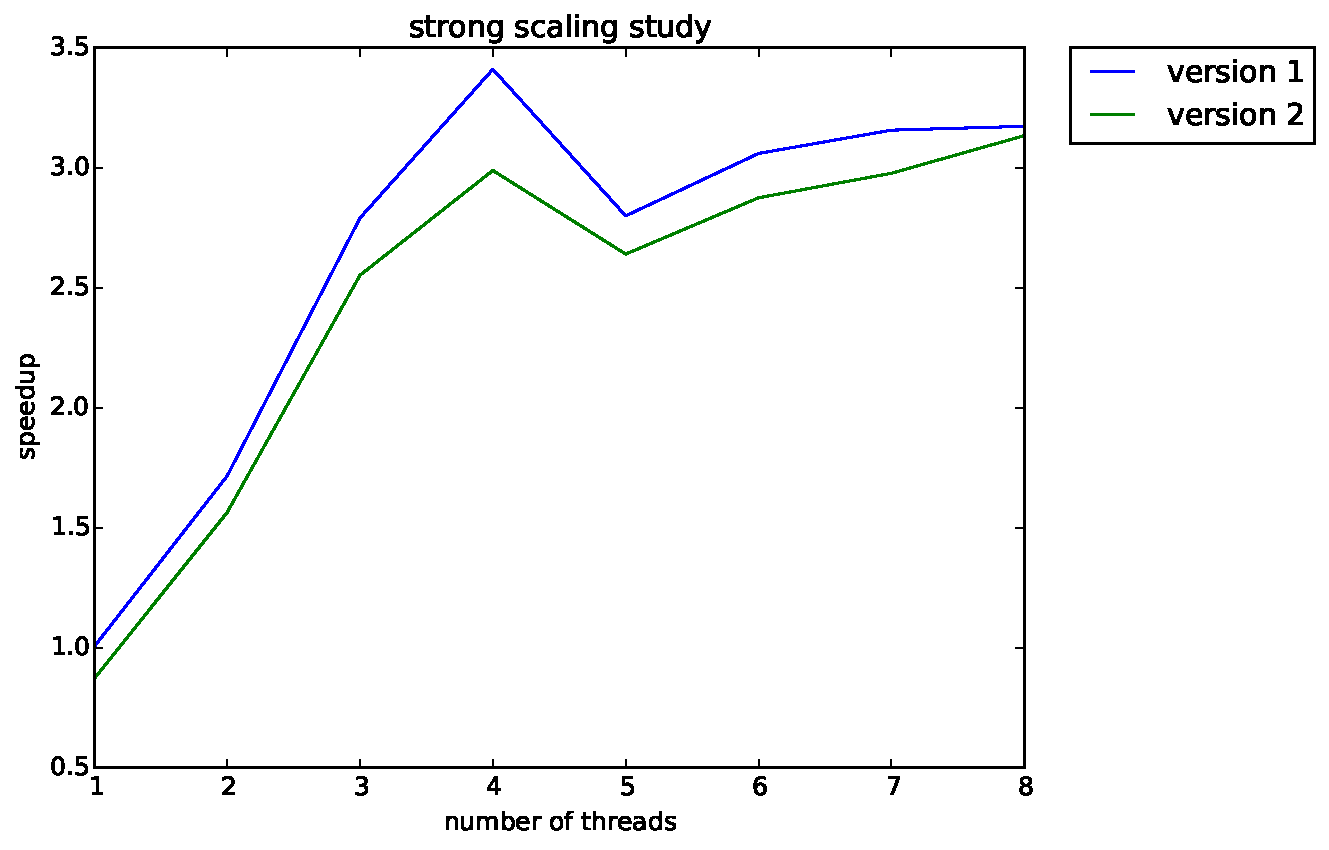
\includegraphics[width=0.85\textwidth] {plots/1_for_strong}
        \end{center}
      \label{aload0}
      \caption{strong scaling}
  \end{subfigure}
  \begin{subfigure}
      \centering
        \begin{center}
      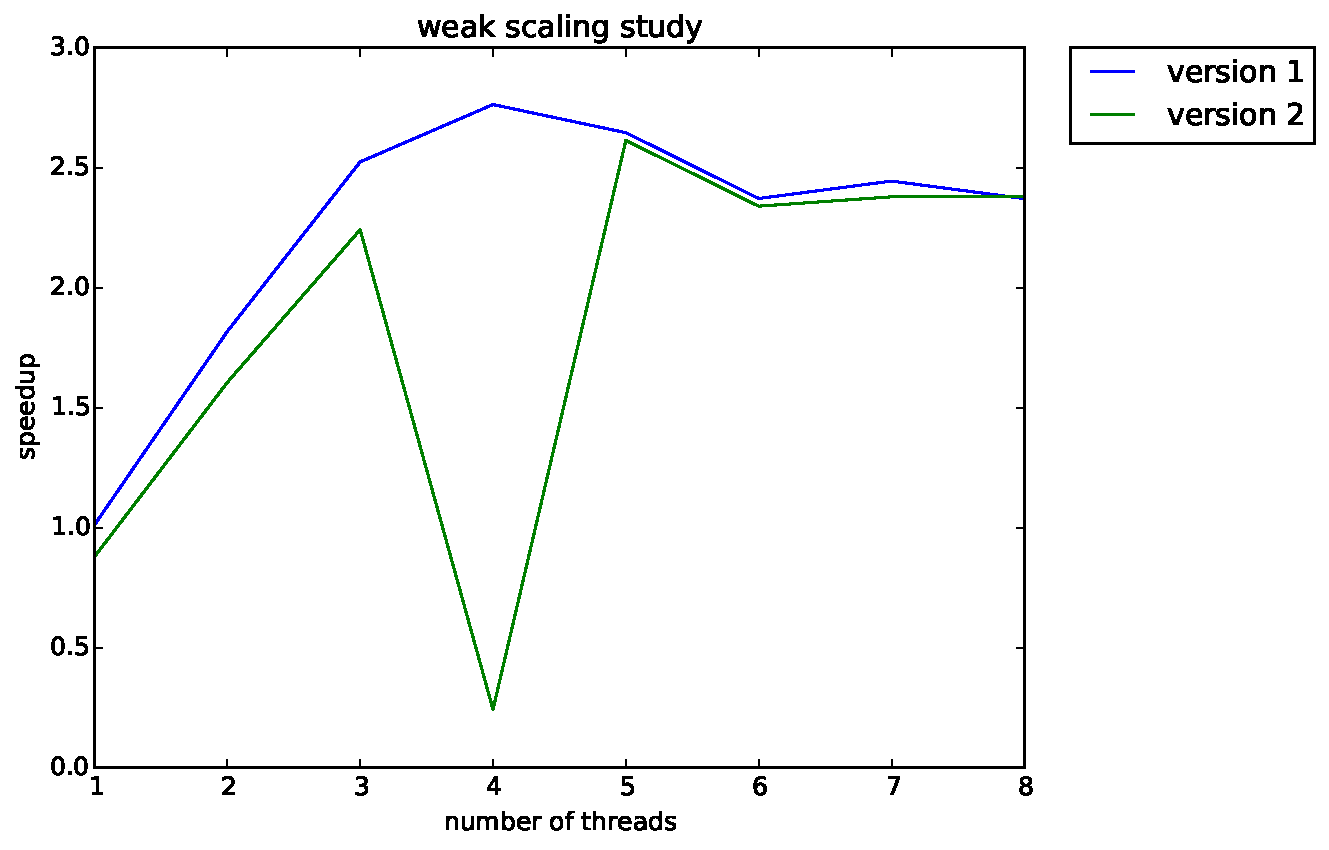
\includegraphics[width=0.85\textwidth] {plots/1_for_weak}
        \end{center}
      \label{aload1}
      \caption{weak scaling}
  \end{subfigure}

\end{figure}

\begin{figure}[!ht]
   \begin{subfigure}
      \centering
        \begin{center}
      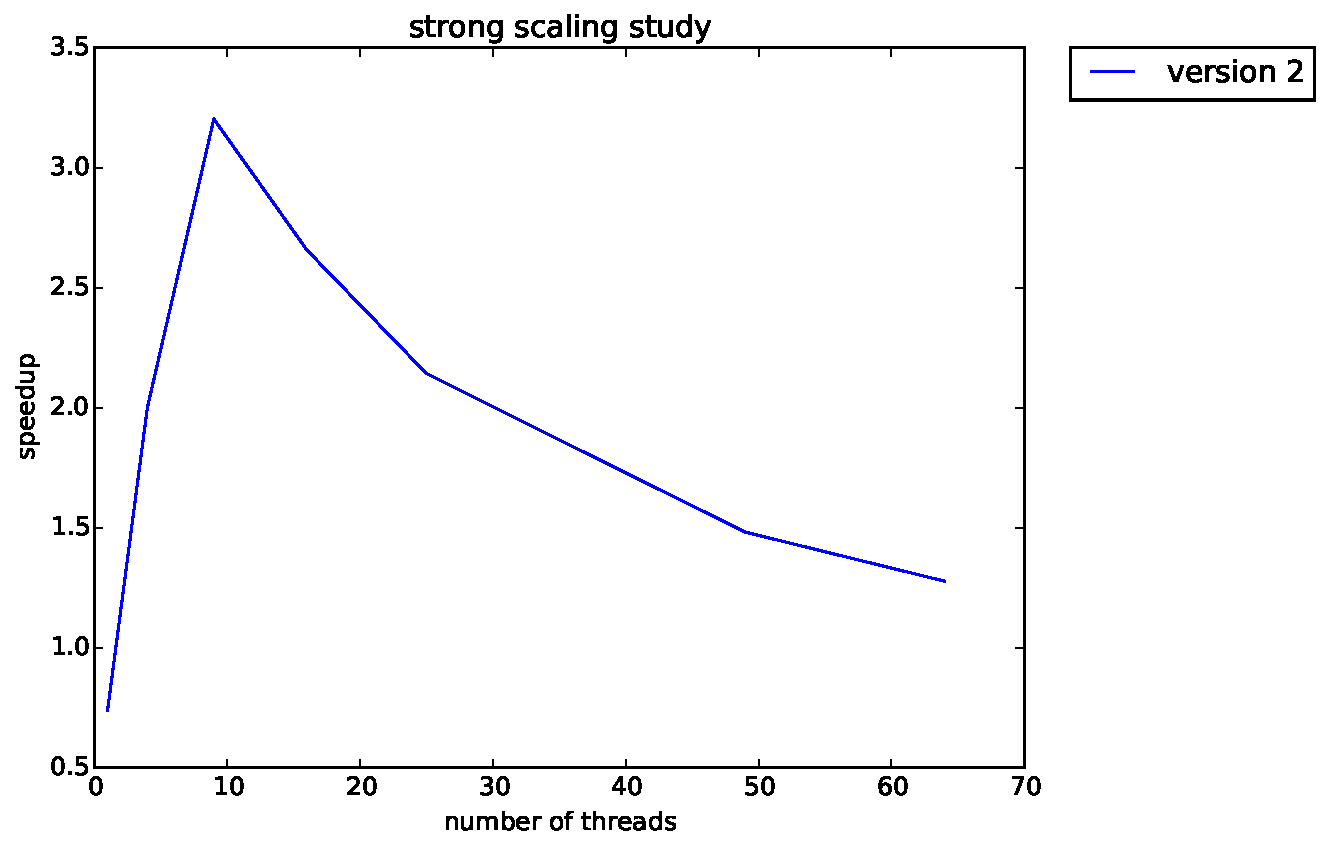
\includegraphics[width=0.85\textwidth] {plots/domain_strong}
        \end{center}
      \label{aload0}
      \caption{strong scaling}
  \end{subfigure}
  \begin{subfigure}
      \centering
        \begin{center}
      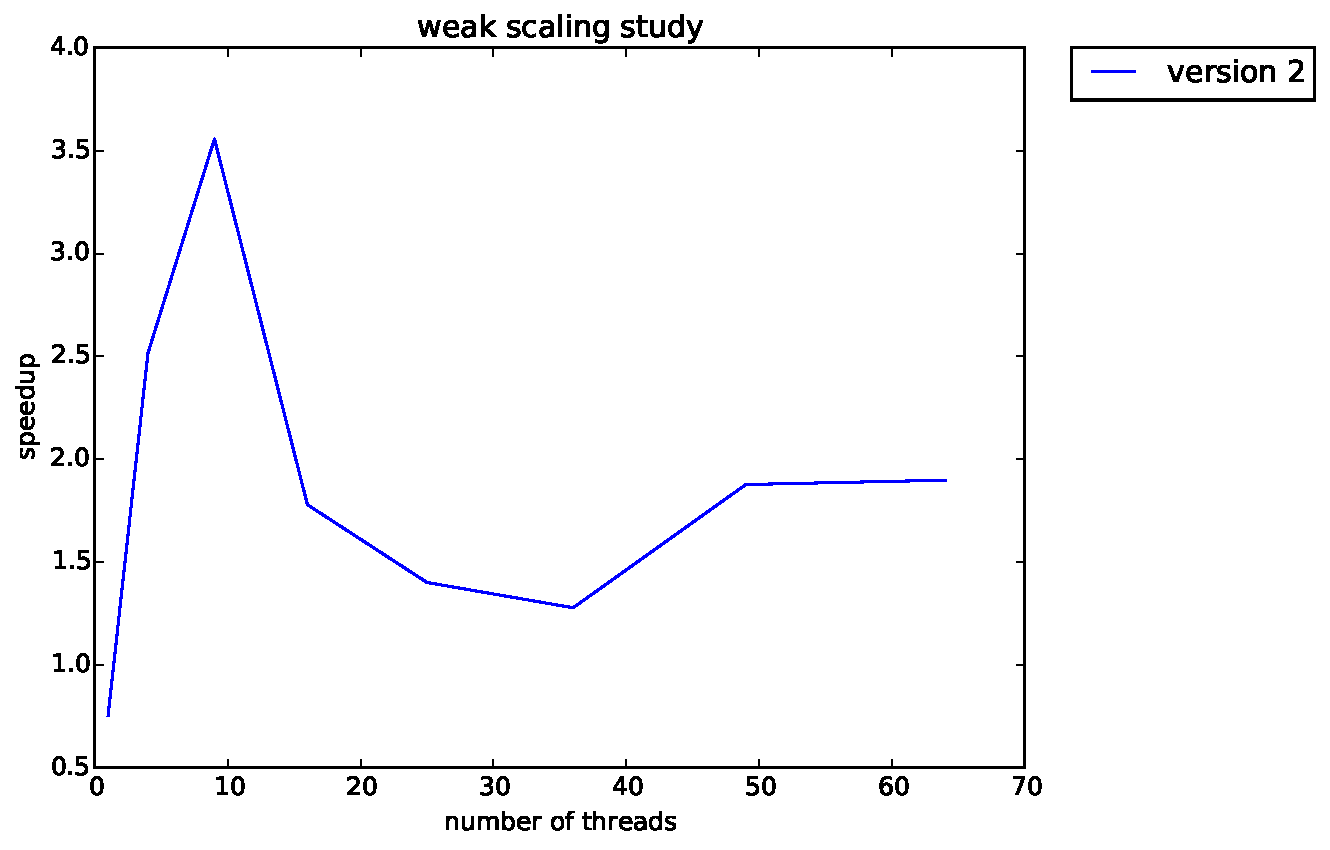
\includegraphics[width=0.85\textwidth] {plots/domain_weak}
        \end{center}
      \label{aload1}
      \caption{weak scaling}
  \end{subfigure}

\end{figure}



\begin{figure}[!ht]
   \begin{subfigure}
      \centering
        \begin{center}
      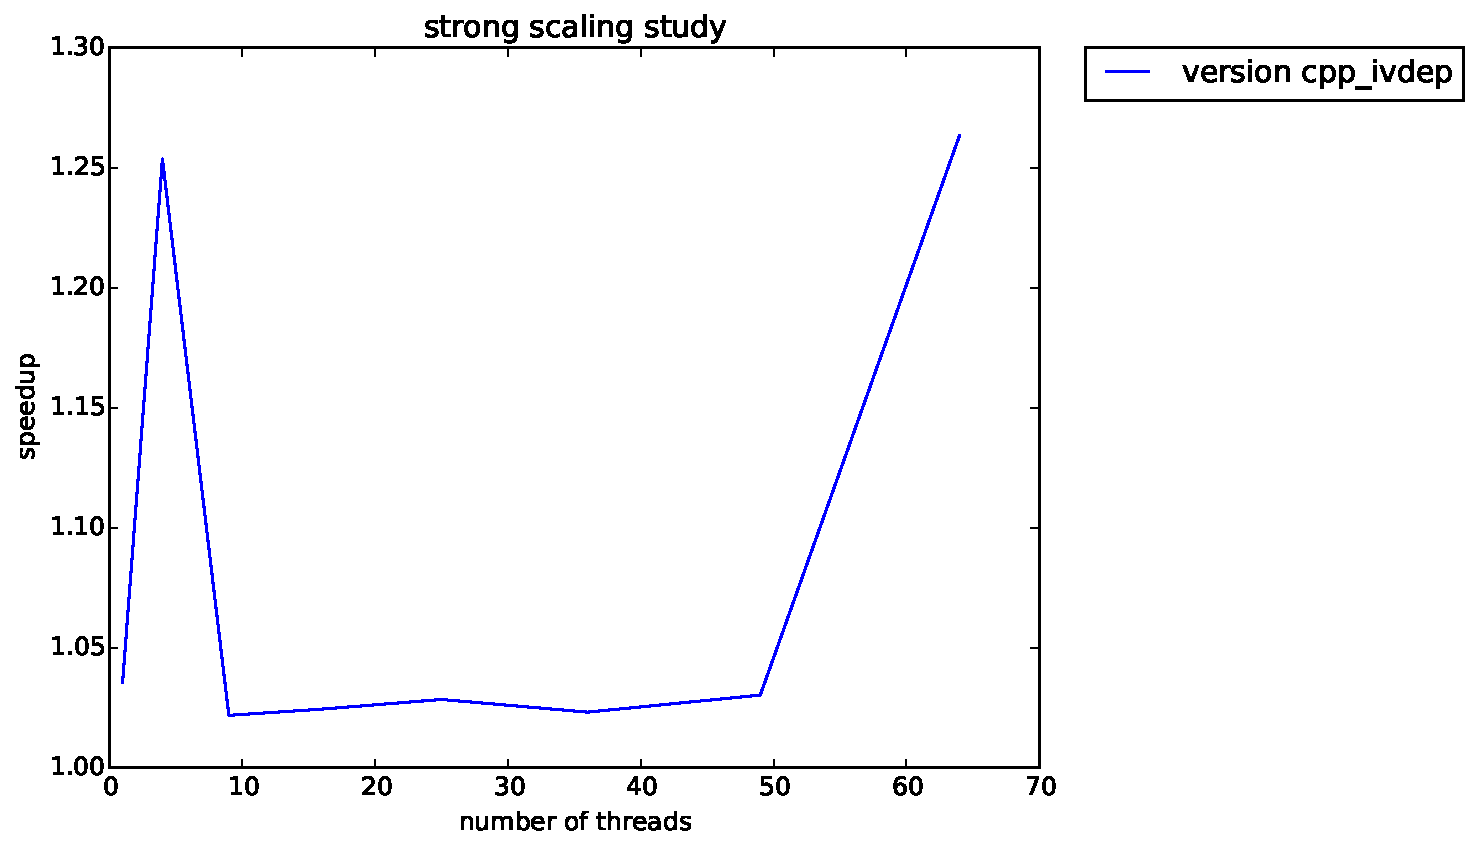
\includegraphics[width=0.85\textwidth] {plots/cpp_strong_ivdep}
        \end{center}
      \label{aload0}
      \caption{strong scaling}
  \end{subfigure}
  \begin{subfigure}
      \centering
        \begin{center}
      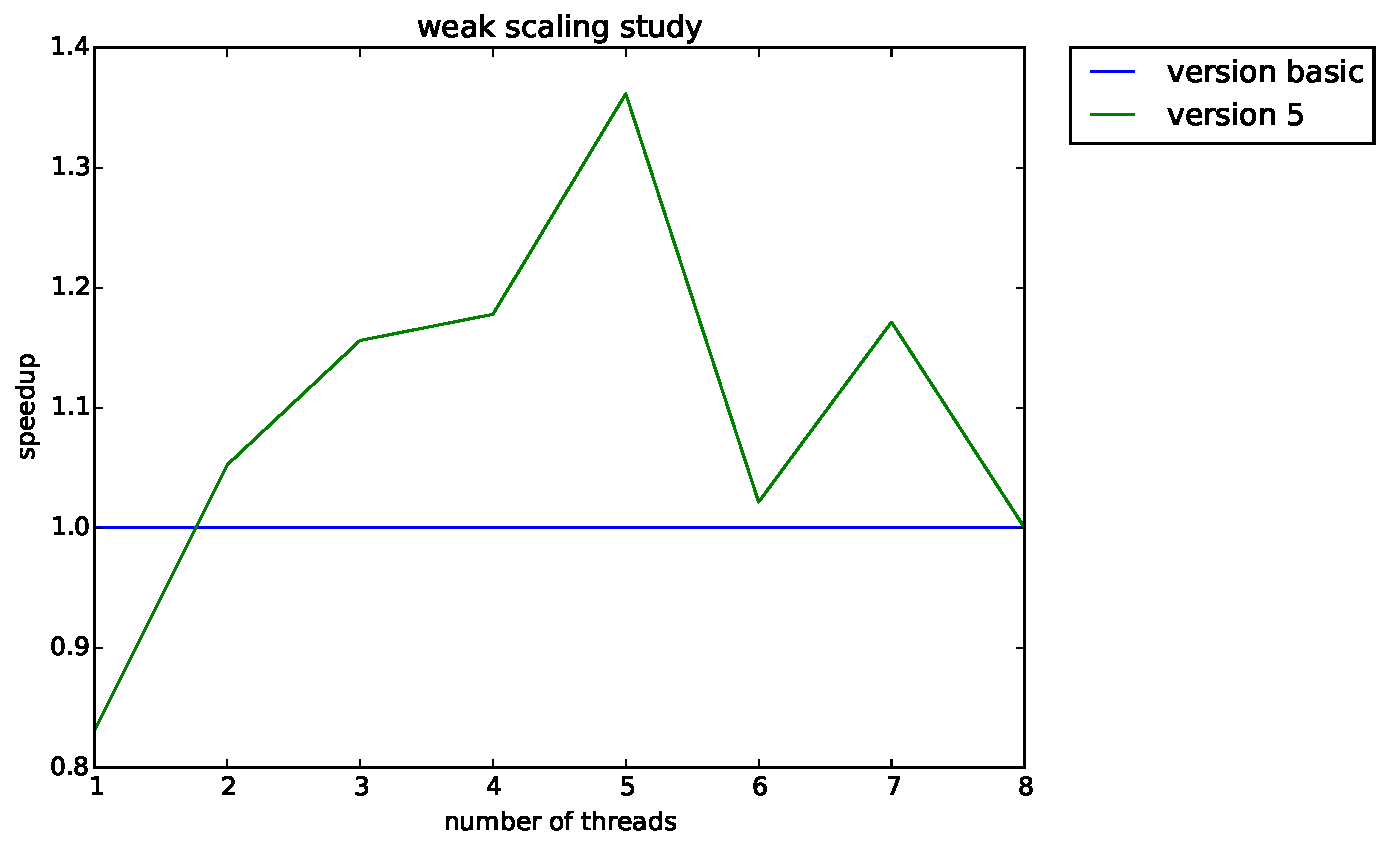
\includegraphics[width=0.85\textwidth] {plots/cpp_weak_ivdep}
        \end{center}
      \label{aload1}
      \caption{weak scaling}
  \end{subfigure}

\end{figure}



\begin{figure}[!ht]
   \begin{subfigure}
      \centering
        \begin{center}
      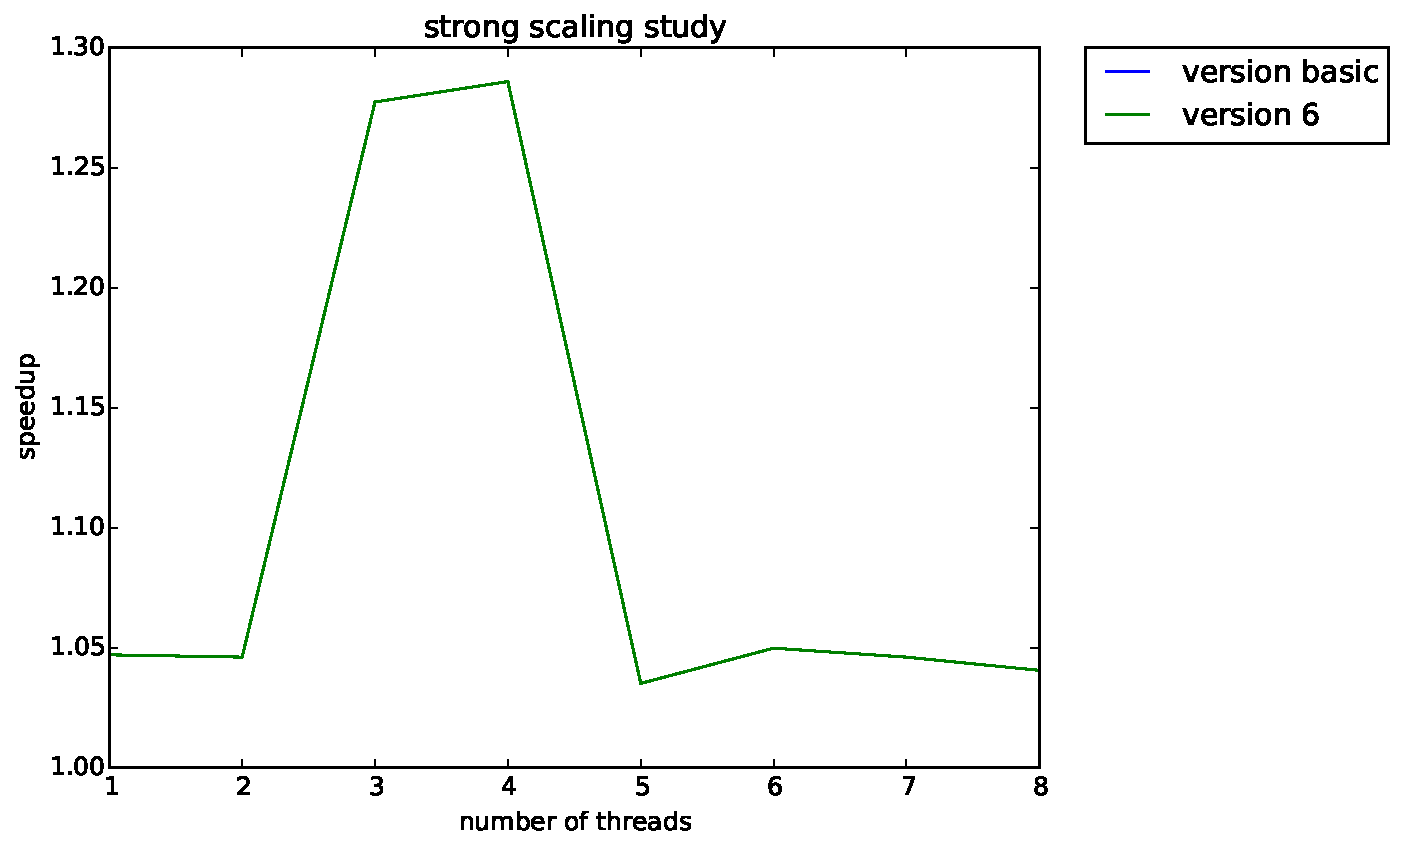
\includegraphics[width=0.85\textwidth] {plots/cpp_strong_ivdep+simd}
        \end{center}
      \label{aload0}
      \caption{strong scaling}
  \end{subfigure}
  \begin{subfigure}
      \centering
        \begin{center}
      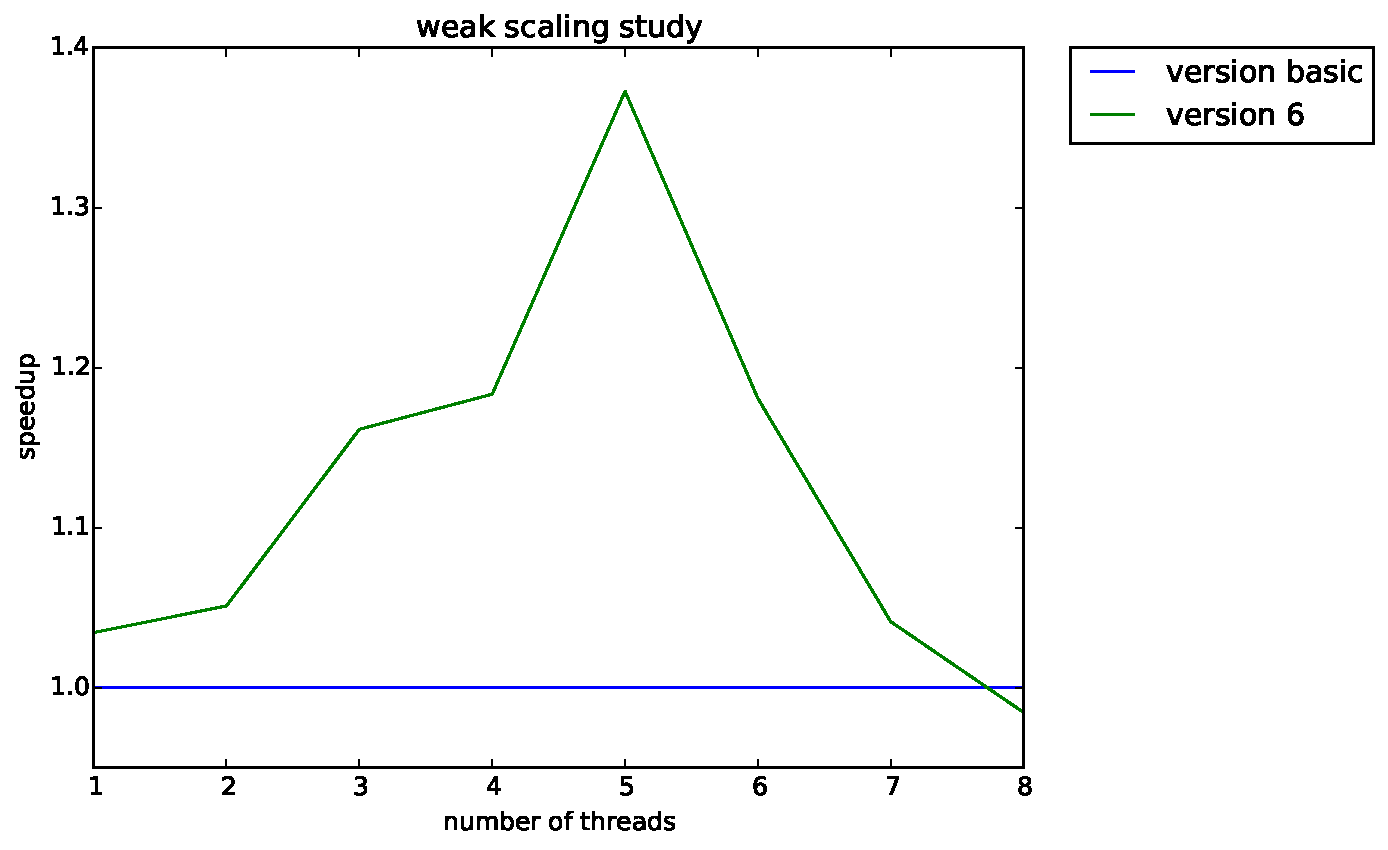
\includegraphics[width=0.85\textwidth] {plots/cpp_weak_ivdep+simd}
        \end{center}
      \label{aload1}
      \caption{weak scaling}
  \end{subfigure}
\end{figure}




\begin{figure}[!ht]
   \begin{subfigure}
      \centering
        \begin{center}
      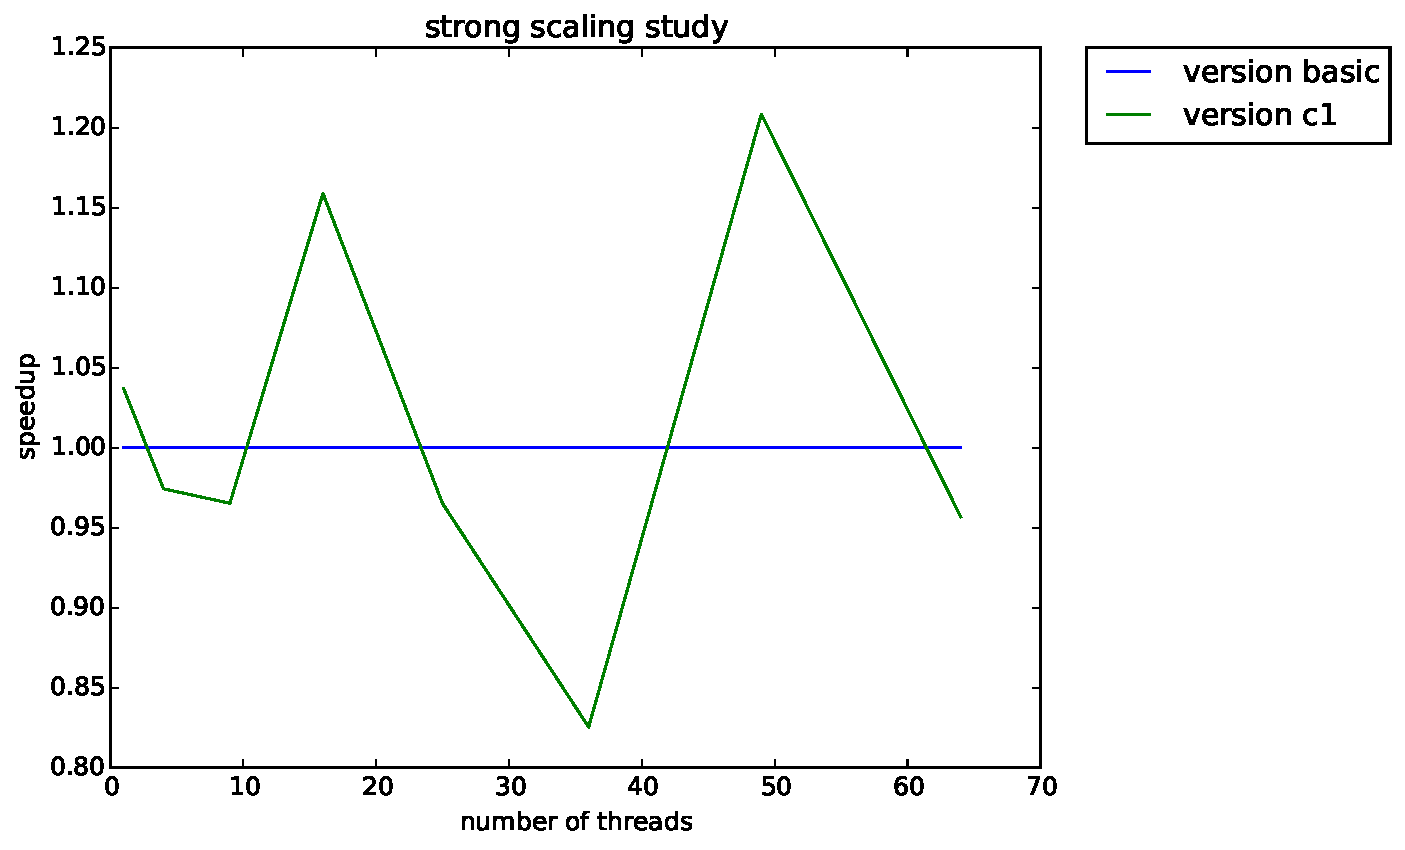
\includegraphics[width=0.85\textwidth] {plots/c_strong_ivdep}
        \end{center}
      \label{aload0}
      \caption{strong scaling}
  \end{subfigure}
  \begin{subfigure}
      \centering
        \begin{center}
      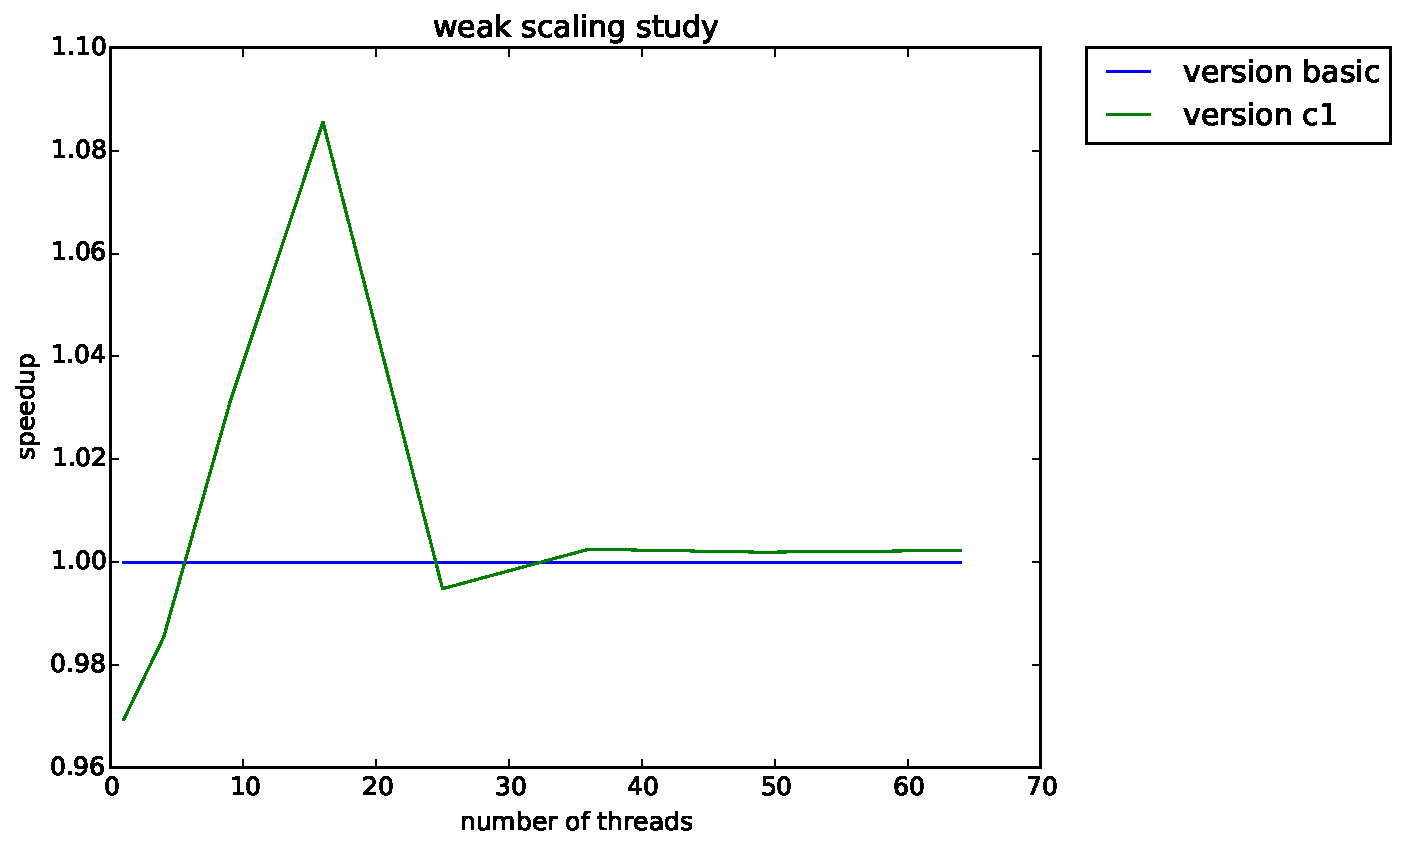
\includegraphics[width=0.85\textwidth] {plots/c_weak_ivdep}
        \end{center}
      \label{aload1}
      \caption{weak scaling}
  \end{subfigure}
\end{figure}




\begin{figure}[!ht]
   \begin{subfigure}
      \centering
        \begin{center}
      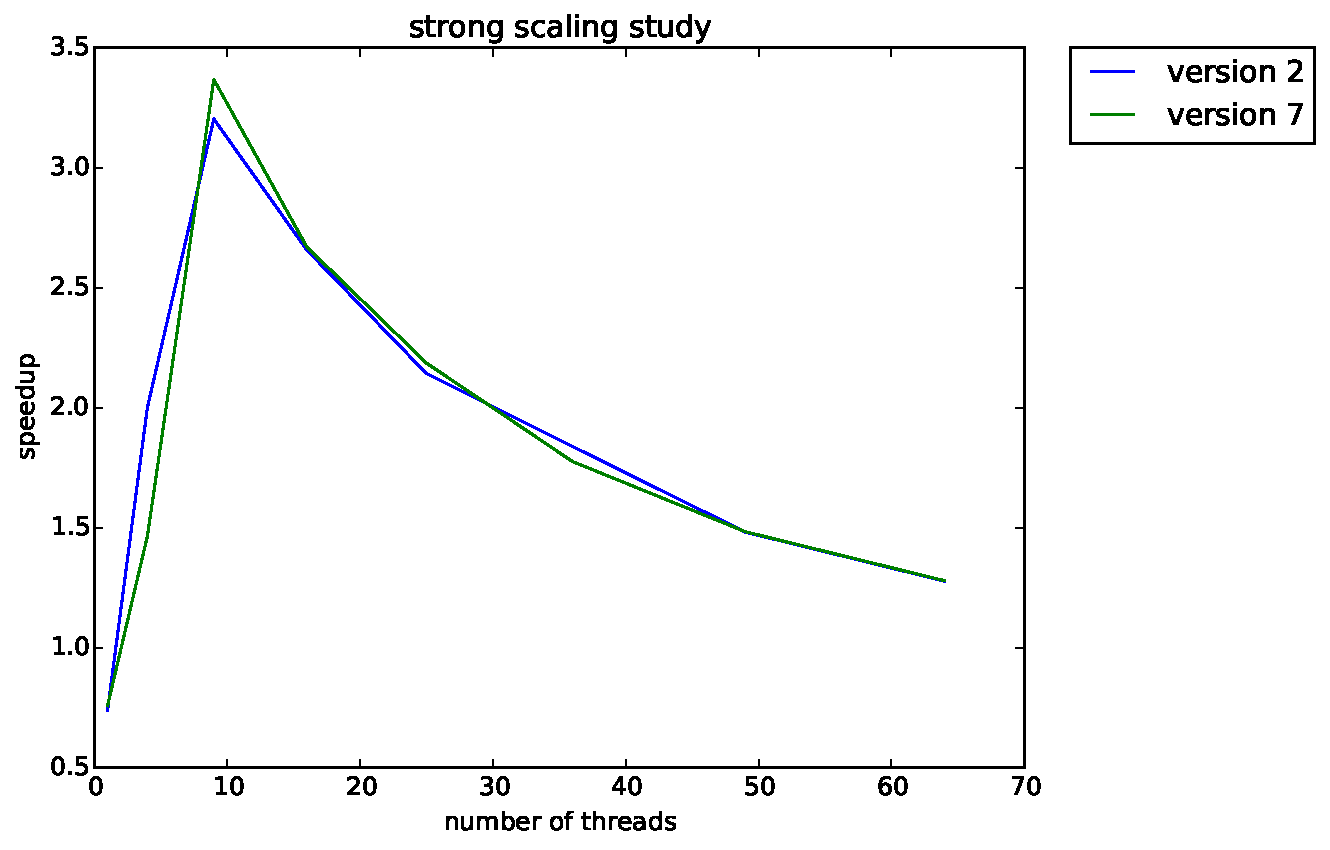
\includegraphics[width=0.85\textwidth] {plots/domain_offload_strong}
        \end{center}
      \label{aload0}
      \caption{strong scaling}
  \end{subfigure}
  \begin{subfigure}
      \centering
        \begin{center}
      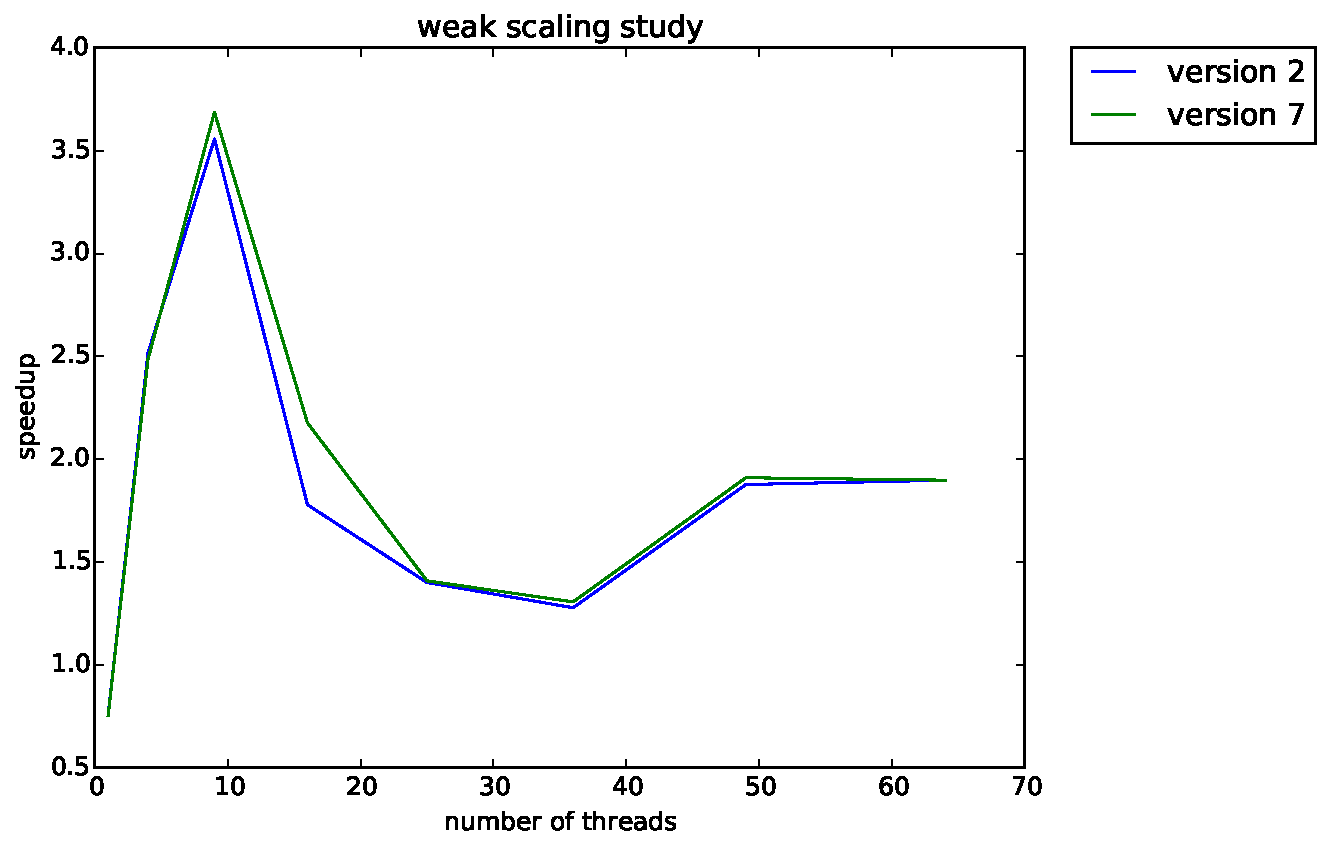
\includegraphics[width=0.85\textwidth] {plots/domain_offload_weak}
        \end{center}
      \label{aload1}
      \caption{weak scaling}
  \end{subfigure}

\end{figure}



\begin{figure}[!ht]
   \begin{subfigure}
      \centering
        \begin{center}
      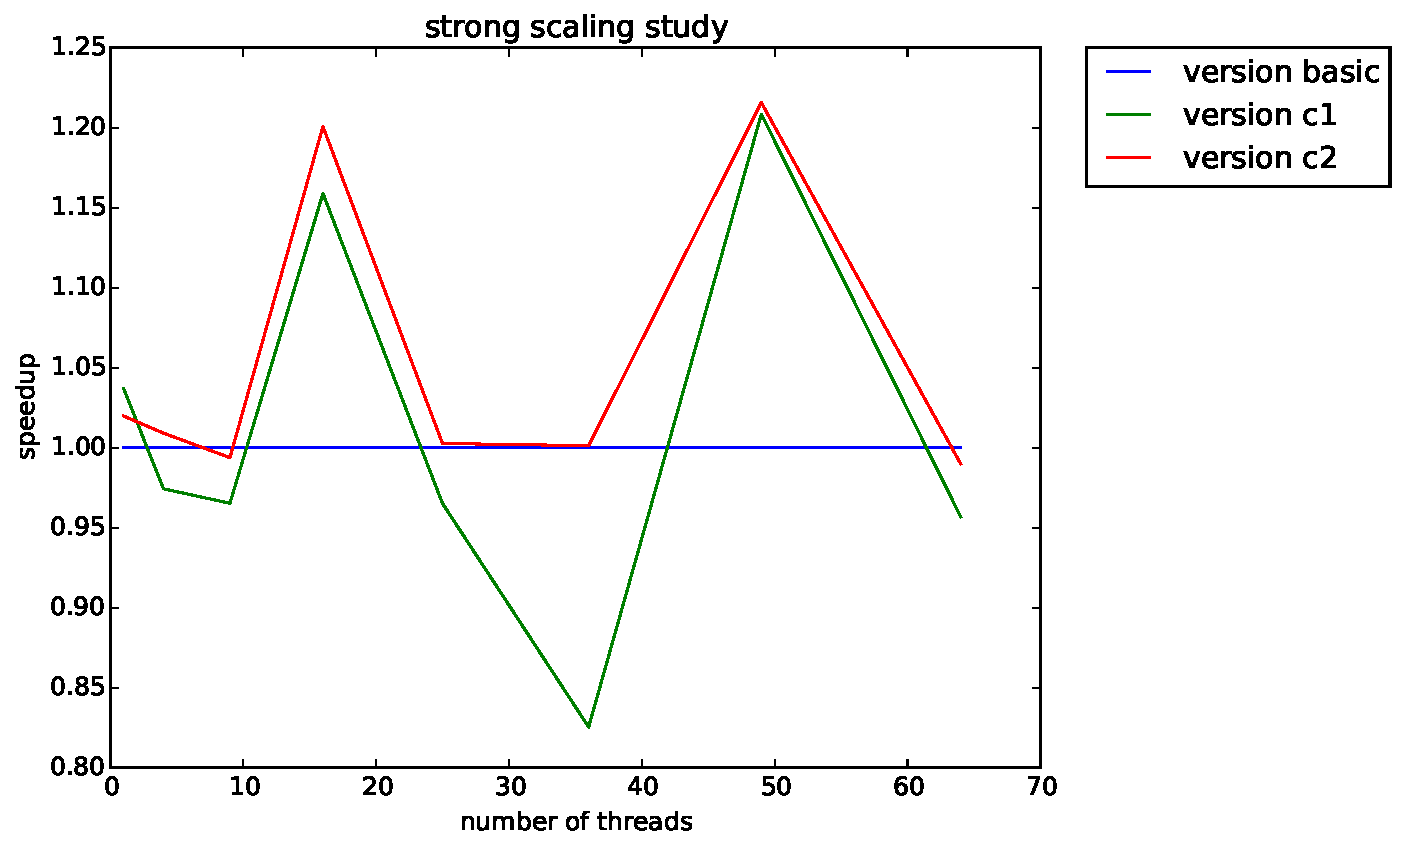
\includegraphics[width=0.85\textwidth] {plots/c_strong_ivdep+simd+flags}
        \end{center}
      \label{aload0}
      \caption{strong scaling}
  \end{subfigure}
  \begin{subfigure}
      \centering
        \begin{center}
      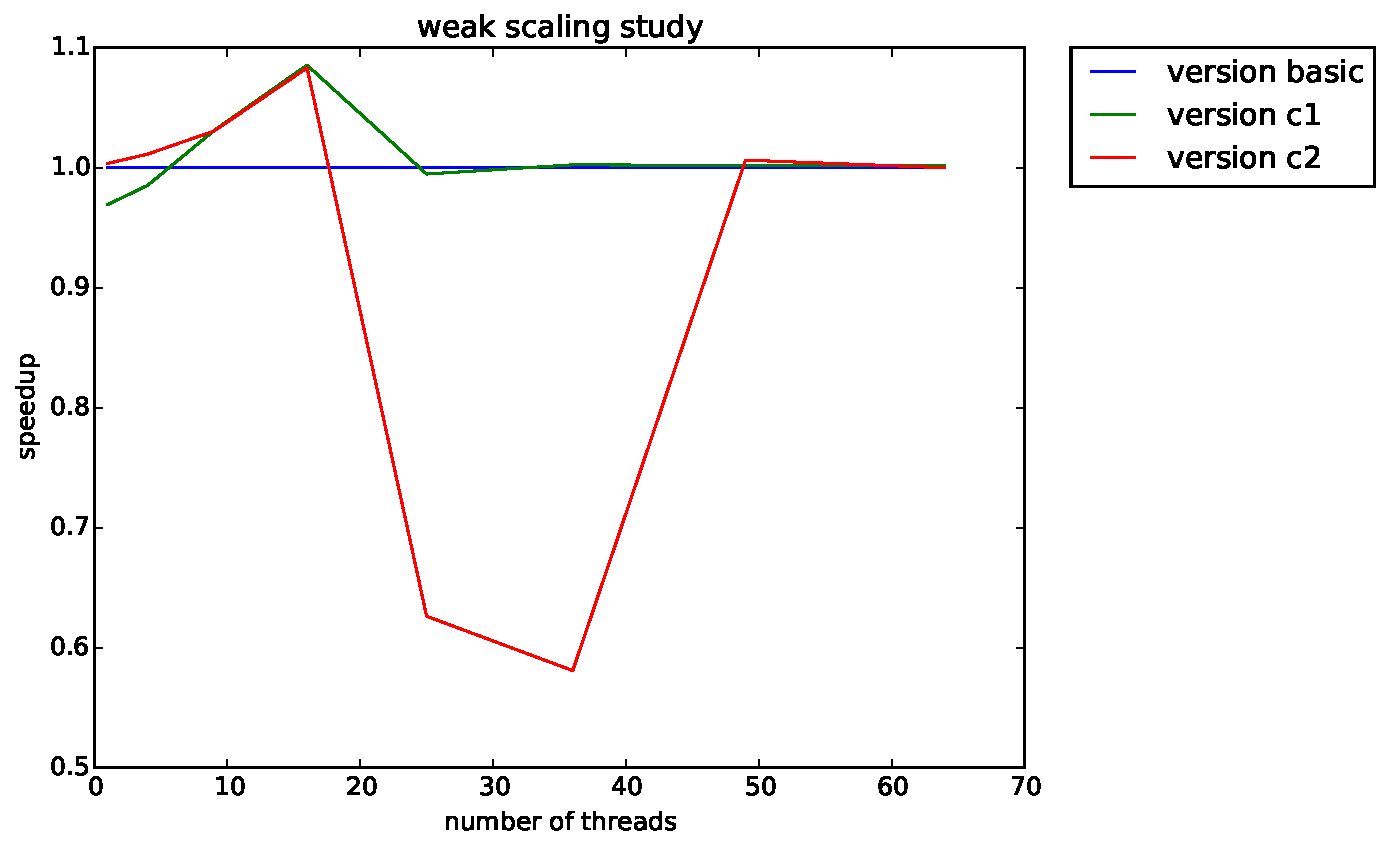
\includegraphics[width=0.85\textwidth] {plots/c_weak_ivdep+simd+flags}
        \end{center}
      \label{aload1}
      \caption{weak scaling}
  \end{subfigure}
\end{figure}

\begin{figure}[!ht]
   \begin{subfigure}
      \centering
        \begin{center}
      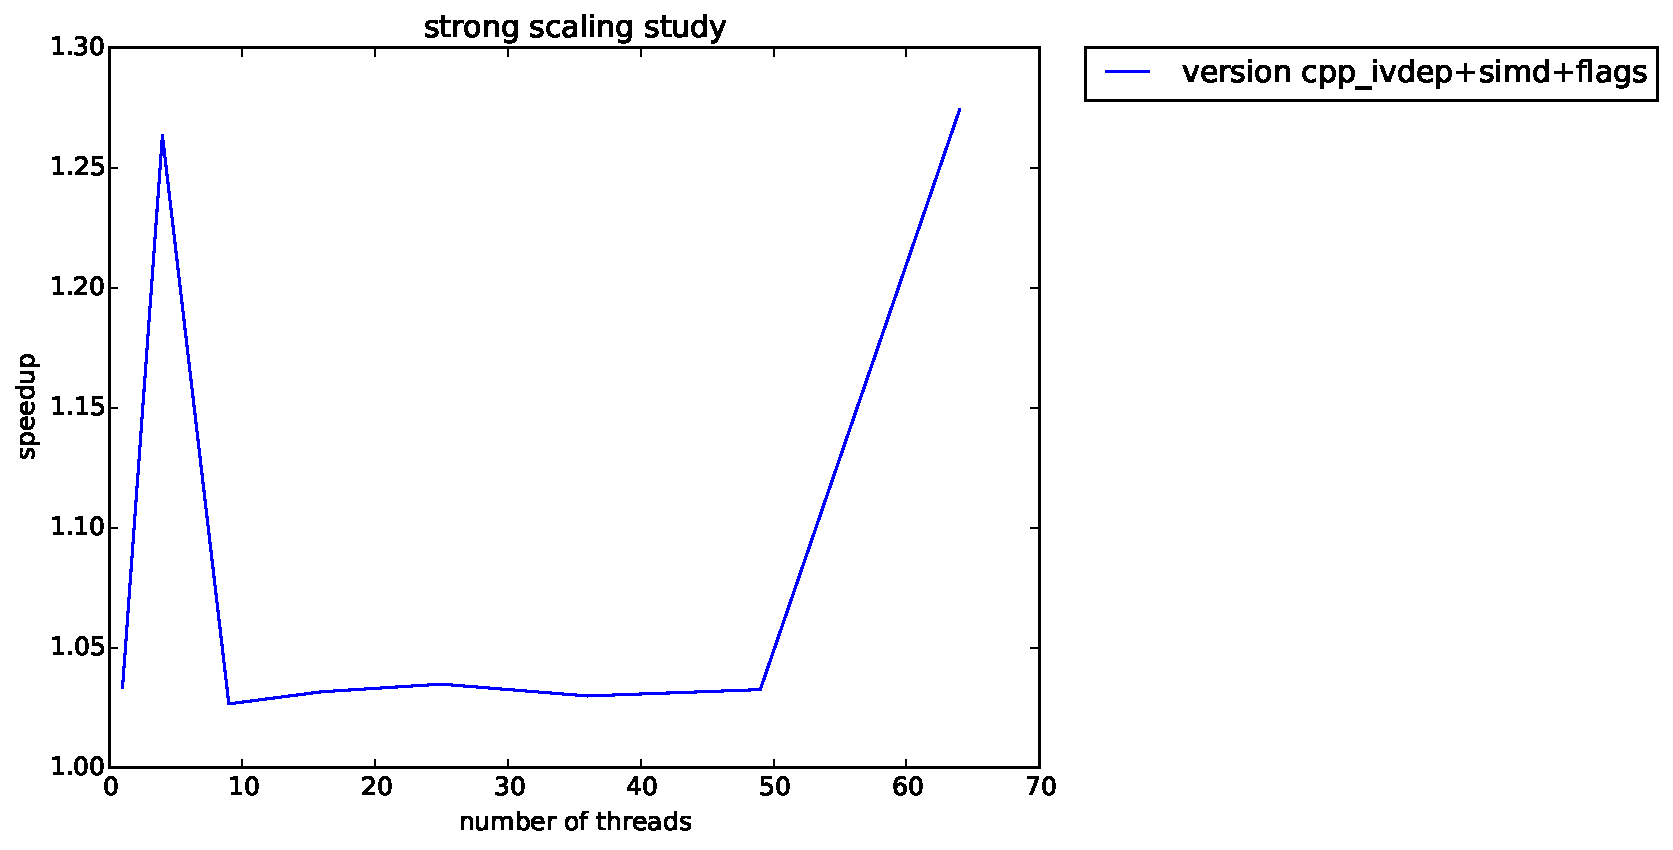
\includegraphics[width=0.85\textwidth] {plots/cpp_strong_ivdep+simd+flags}
        \end{center}
      \label{aload0}
      \caption{strong scaling}
  \end{subfigure}
  \begin{subfigure}
      \centering
        \begin{center}
      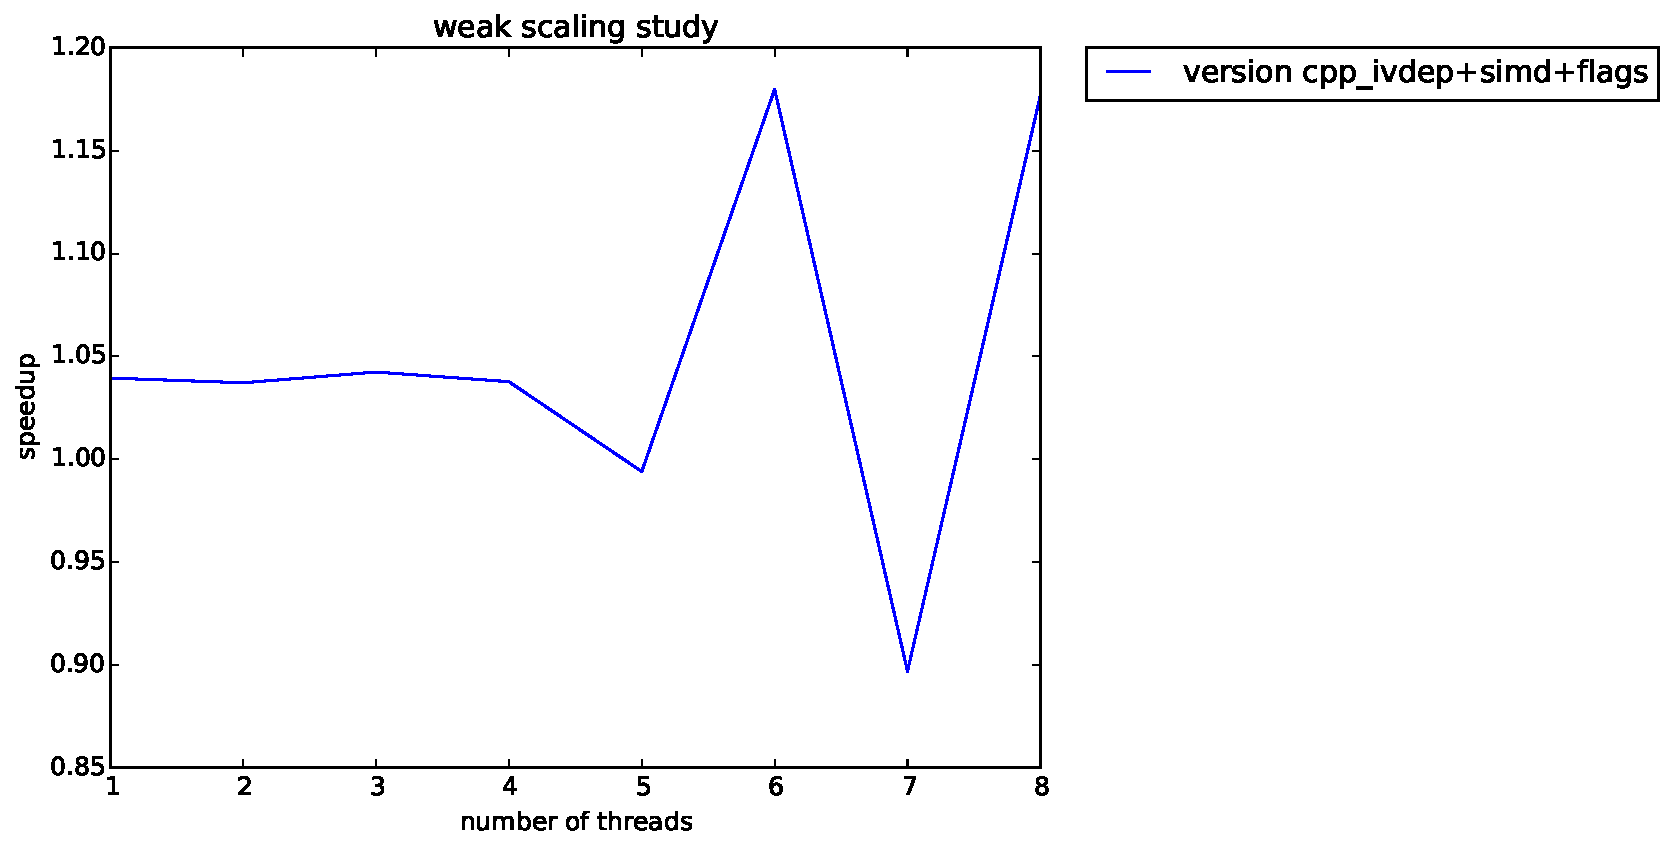
\includegraphics[width=0.85\textwidth] {plots/cpp_weak_ivdep+simd+flags}
        \end{center}
      \label{aload1}
      \caption{weak scaling}
  \end{subfigure}
\end{figure}

\end{document}





